\subsection{Import und Verarbeitung des FEM-Gitters}
In diesem Abschnitt wird kurz der Import und die Verarbeitung des FEM-Gitters beschrieben. Dabei wird genauer auf die Methodik zur korrekten Interpretation der Randbedingungen eingegangen. So erfordert zum Beispiel die Berechnung des Elementgleichungssystems im 2D-Fall ein Kurvenintegral entlang des neumannschen Randes, wobei sich diese aus mehreren Dreiecksseiten zusammensetzt. Somit ist es zwingend notwendig aus dem generierten Gitter herauszulesen welche Seite oder Seiten der entsprechenden Elemente am neumannschen Rand liegen.

\subsubsection{Import des Gitters}
Wie schon zuvor erwähnt benötigt die Software eine Gitterdatei der Version 2. Dabei handelt es sich um ASCII-codierte Dateien mit \textbf{mindestens} folgenden Informationen:

\begin{itemize}
	\item \textbf{Format der Datei im Abschnitt \textit{\$MeshFormat\$}}. Sie Software unterstützt nur Dateien der Version 2.2.0.8
	
	\item \textbf{Informationen über die 'Physical Groups' der Problemgeometrie im Abschnitt \textit{\$Physical Names\$}}. Dabei gibt der erste Eintrag des Abschnitts die Anzahl der \textit{Physical Groups} an. Jeder weitere Eintrag steht für eine \textit{Physical Group}, definiert durch jeweils drei Parameter:
	\begin{enumerate}
		\item \textbf{Dimension der \textit{Physical Group}}. 1: 1-dimensional (Kurve), 2: 2-dimensional (Fläche)
		\item \textbf{ID}. Jede Gruppe bekommt eine positive Ganzzahl zur eindeutigen Identifikation zugewiesen.
		\item \textbf{Name}. Jener Name der der \textit{Physical Group} bei der Erstellung zugewiesen wurde.
	\end{enumerate}

	\item \textbf{Daten der Elementkonten des Gitters im Abschnitt \textit{\$Nodes\$}}. Der erste Eintrag gibt wieder die Anzahl der Knoten an, jeder weitere Eintrag steht für einen Knoten, wobei die erste Zahl eine positive Ganzzahl zur eindeutigen Identifizierung des Knotens darstellt. Die weiteren drei Einträge sind Gleitkommazahlen für die x-, y- und z-Koordinaten.
	
	\item \textbf{Definitionen der finiten Elemente im Abschnitt \textit{\$Elements\$}}. Der erste Eintrag gibt die Anzahl der finiten Elemente an, und jede weiter Zeile definiert ein Element nach dem folgenden Schema:
	\begin{enumerate}
		\item \textbf{ID}. Eine positive Ganzzahl zur eindeutigen Identifikation des Elements.
		\item \textbf{Typ des Elements}. Gmsh kennt viele verschiedene Elementtypen. Für eine vollständige Liste sei auf die Dokumentation von Gmsh verwiesen (\cite{gmsh_website}). Da sie Software dreieckige finite Elemente bis zur Ordnung 3 unterstützt sind hier folgende Einträge möglich:
		\begin{itemize}
			\item 2: 2-knotige lineare Linie/Kurve
			\item 3: 3-knotiges lineares Dreieckselement
			\item 8: 3-knotige quadratische Line/Kurve
			\item 9: 6-knotiges quadratisches Dreieckselement
			\item 26: 4-knotige kubische Linie/Kurve
			\item 21: 10-knotiges kubisches Dreieckselement
		\end{itemize}
		\textbf{Anmerkung:} In Zukunft könnten weitere Elementtypen unterstützt werden.
		\item \textbf{Anzahl der \textit{Physical Tags}}. 
		\item 'Physical Tage'. Auch hier sei zu deren genauen Bedeutung auf die Dokumentation von Gmsh \cite{gmsh_website} verwiesen. Standardmäßig ist der erste Eintrag nach der Anzahl der \textit{Physical Tags} die ID der \textit{Physical Group} der das Element angehört. Alle Weiteren \textit{Tags} werden nicht benötigt.
		\item \textbf{IDs der Elementknoten}. Je nach Elementtyp findet sich hier eine unterschiedliche Anzahl an Einträgen. Es ist zu beachten dass Gmsh die Reihenfolge der Knoten der finiten Elemente anders als das FEM-Tool definiert. Hierbei sei auf die Gmsh Dokumentation, Abschnitt 9.2 verwiesen. Die Definitionen des FEM-Tools finden sich in diesem Dokument unter Abschnitt \ref{sec:finite_elements_and_shape_functions}. Es ist somit ein Umordnen der Knoten notwendig, was jedoch von der Software automatisch beim Import durchgeführt wird.
	\end{enumerate}
\end{itemize}

Eine beispielhafte Gitterdatei zu dem in Abbildung \ref{fig:neumann_boundary_assignment} gezeigten Beispiel findet sich in Listing \ref{fig:example_mesh_file}.


\subsubsection{Verarbeitung der Gitterinformation}
Nach erfolgreichem Import der Gitterinformation sind zur vollständigen Definition des Problems die Randbedingungen des Problems, sowie Materialeigenschaften und weitere Informationen wie zum Beispiel Quellen (freie Raumladungen etc.) den einzelnen Elementen zuzuordnen: \newline

\begin{itemize}
	\item \textbf{Knoten am dirichletschen Rand}. Das Potential des entsprechenden Elementknotens ist bereits vorgegeben, was bei der Berechnung des Elementgleichungssystems entsprechend berücksichtigt werden muss.
	\item \textbf{Knoten und Seiten am neumannschen Rand}. Wie aus (\ref{eq:right_side_e_static}) ersichtlich erfordert die Berechnung von $r_j$ ein Integral über die neumannsche Randfläche, welches im zweidimensionalen Fall zu einem Kurvenintegral entartet. Dazu ist es notwendig zu wissen welche Dreiecksseiten der Elemente am neumannschen Rand liegen.
	\item \textbf{Materialeigenschaften im Element}. Wie in \ref{eq:k_ij_e_static} ersichtlich ist es notwendig $\epsilon_x$ und $\epsilon_y$ für jedes Element zu kennen. Die Deklaration von $\epsilon_x$ und $\epsilon_y$ erfolgt in einem separaten File. Die Zuordnung zum entsprechenden Element erweist sich als trivial da jeder Elementdefinition die ID der entsprechenden 2D \text{Physical Group} beiliegt.
	\item \textbf{Quellen im Element}. Analog zu den Materialeigenschaften verhält es sich mit den Quellen innerhalb eines Elements. Die Quellen kommen z.B. bei der Berechnung von (\ref{eq:right_side_e_static}) als Parameter $\rho$ zum Tragen. Auch hier erweist sich die Zuordnung wieder als trivial.
\end{itemize}

Die Zuordnung der Knoten und Dreiecksseiten an den Rändern des Problems wird im folgenden Kapitel beschrieben.

\subsubsection{Zuordnung der Knoten am dirichletschen- und Dreiecksseiten am neumannschen Rand}
\label{sec:rb_assignment}
\textbf{Knoten am dirichletschen Rand:}
\begin{enumerate}
	\item Die Elementknoten am dirichletschen Rand sind zu ermitteln. Dies ist ohne weitere Umschweife möglich, da die Definition der Kurvenelemente in der Gitterdatei bereits die ID der entsprechenden \textit{Physical Group} enthält. Somit liegen alle Knoten von Kurvenelementen mit der Entsprechenden ID am dirichletschen Rand.
	
	\item Alle Dreieckselemente die nun mindestens einen der vorher ermittelten Knoten enthalten sind zu bestimmen. Jedem dieser Knoten wird anschließend der entsprechende Randwert zugeordnet.
\end{enumerate}

\textbf{Dreiecksseiten am neumannschen Rand:}
\begin{enumerate}
	\item Zur Ermittlung der Elementknoten an Rand wird der Algorithmus von oben angewendet.
	\item Die Bestimmung der Dreiecksseiten am neumannschen Rand erfolgt durch Vergleich von der Elementknoten mit den Knoten am Rand:\newline
	Je nach Elementtyp ist eine Dreiecksseite durch 2, 3 oder 4 Knoten definiert. Siehe dazu Abschnitt \ref{sec:finite_elements_and_shape_functions}. Liegt ein Dreieckselement am neumannschen Rand, so stimmen alle Knoten einer oder mehrerer Seiten mit entsprechend vielen Knoten am Rand überein. Hierbei ist zu erwähnen dass auch bei mehr als 2 Knoten pro Seite die ganze Seite am Rand liegen muss. \newline
	Durch die Verwendung von isoparametrischen finiten Elementen sind im lokalen Koordinatensystem nur drei verschiedene Kurvenintegrale möglich, was eine statische Zuordnung eines Kurvenintegrals zu jeder Dreiecksseite ermöglicht. Zu diesem Zweck wird jeder Dreiecksseite eine Nummer zugewiesen:
	\begin{itemize}
		\item Die Dreiecksseite auf der $\xi$-Achse sei definiert als \textit{Seite 1}.
		\item Die Dreiecksseite auf der $\eta$-Achse sei definiert als \textit{Seite 2}.
		\item Die verbleibende Seite sei definiert als \textit{Seite 3}
	\end{itemize}
	\begin{figure}[H]
		\begin{center}
			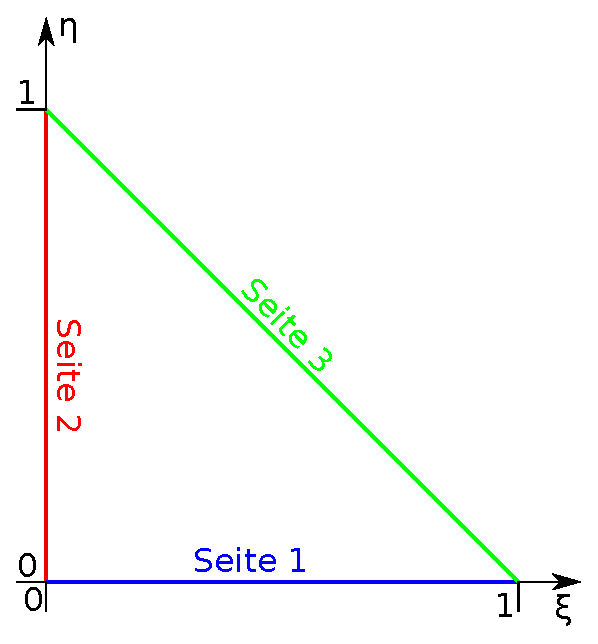
\includegraphics[scale=0.65]{pics/triangle_side_assignment.eps}
		\end{center}
		\caption{Zuordnung der Dreiecksseiten}
		\label{fig:triangle_side_assignment}
	\end{figure}
	\item Zu guter Letzt werden noch den Dreiecksseiten am Rand den Wert der Randbedingung (in (z.B. $\sigma$ aus \ref{eq:right_side_e_static}) ) zugeordnet.
\end{enumerate}

Um die in diesem Abschnitt gezeigten Zusammenhänge zu verdeutlichen, wird die Zuordnung der Dreiecksseiten zum neumannschen Rand anhand des in Abbildung \ref{fig:neumann_boundary_assignment} gezeigten Beispiels verdeutlicht. Eine Beispielhafte Gitterdatei ist in Listing \ref{fig:example_mesh_file} gezeigt.\newline

\textbf{Anmerkung:} Die Gitterdatei aus Listing \ref{fig:example_mesh_file} beschreibt keineswegs ein vollständig definiertes Problem. Sie dient lediglich der Veranschaulichung der Vorgangsweise bei der Zuordnung von Knoten und Seiten an den Problemrändern.

\lstinputlisting[frame=single, backgroundcolor=\color{lightgray}, basicstyle=\ttfamily\footnotesize, caption = {Exemplarische Gitterdatei}, label={fig:example_mesh_file}, captionpos=b ]{neumann_boundary_assignment_example_mesh_file.txt}

\begin{figure}[htbp]
	\begin{minipage}[t]{0.45\textwidth}
	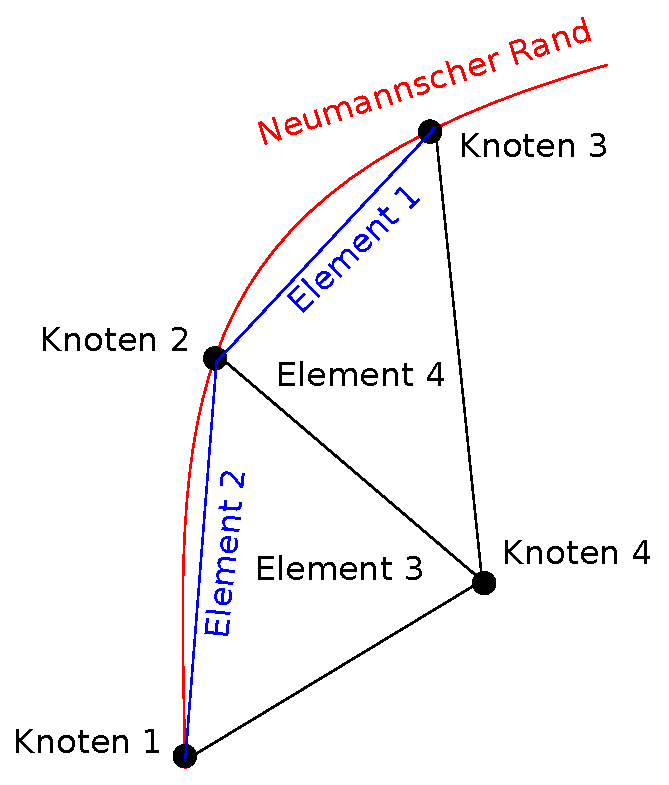
\includegraphics[scale=0.65]{pics/neumann_boundary_assignment.eps}
	\caption{Zuordnung der Dreiecksseiten}
	\label{fig:neumann_boundary_assignment}
	\end{minipage}
	\hfill
	\begin{minipage}[t]{0.45\textwidth}
	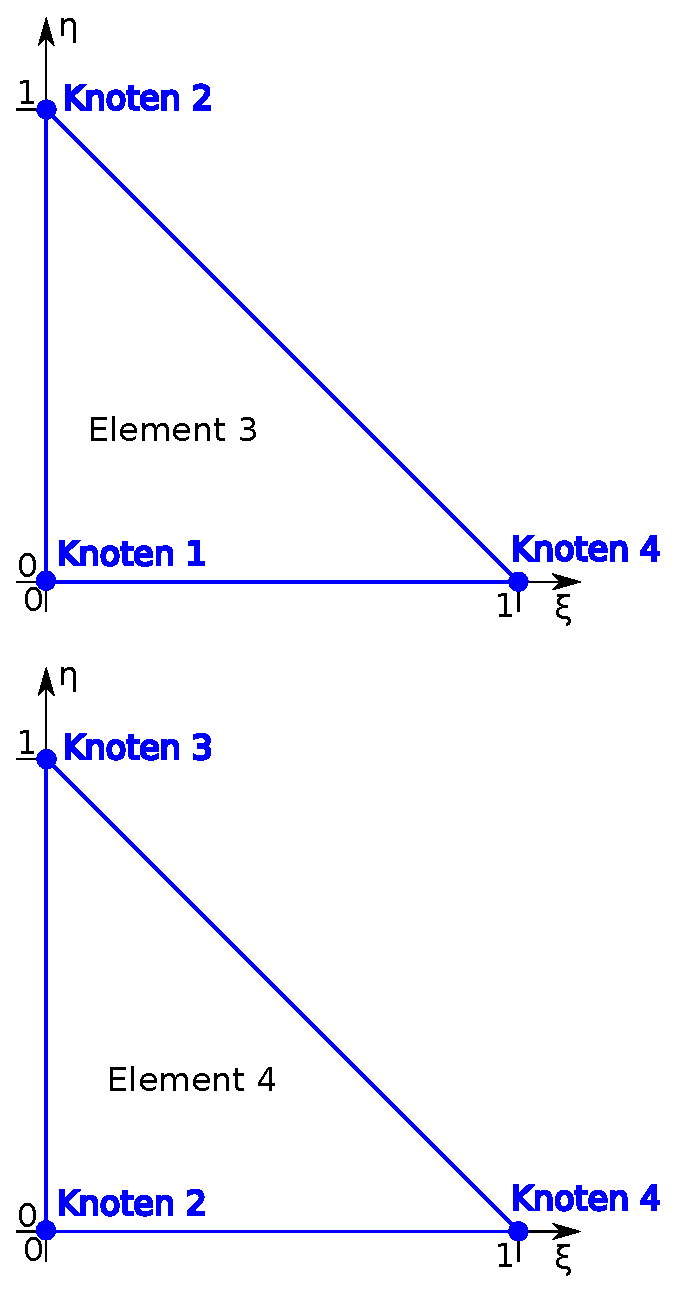
\includegraphics[scale=0.5]{pics/neumann_boundary_assignment_elements_3_4.eps}
	\caption{Elemente 3 und 4 im lokalen Koordinatensystem}
	\label{fig:neumann_boundary_assignment_elements_3_4}
	\end{minipage}	
\end{figure}	

Wie aus Code \ref{fig:example_mesh_file} ersichtlich, setzt sich die Geometrie aus 4 Knoten und 4 Elementen zusammen. Abbildung \ref{fig:neumann_boundary_assignment_elements_3_4} zeigt die Dreieckselemente 3 und 4 in ihrem lokalen Koordinatensystem. 

Wie mit Hilfe von Abbildung \ref{fig:triangle_side_assignment} zu erkennen ist, liegt Element 3 mit Seite 1, und Element 4 mit Seite 2 am neumannschen Rand. Der oben beschrieben Algorithmus wird nun auf dieses Beispiel angewandt um dessen Funktion zu erklären.\newline
\begin{enumerate}
	\item Die Elemente 1 und 2 sind, wie aus Code \ref{fig:example_mesh_file} ersichtlich der \textit{Physical grup} 1 zugeteilt. (Vierter Eintrag in den beiden Elementdefinitionen). Somit ist nun bekannt dass die Knoten 1, 2 und 3 am neumannschen Rand liegen.
	\item Die lokalen Knoten 1 und 2 von Element 3 stimmen mit den globalen Knoten 1 und 2 am neumannschen Rand überein, womit sich nun feststellen lässt dass Element 3 mit Seite 1 am neumannschen Rand liegt.
	\item Selbiges wir nun für Element 4 durchgeführt. Die lokalen Knoten 2 und 3 stimmen mit den globalen Knoten 2 und 3 überein, womit sich feststellen lässt dass Element 4 mit Seite 2 am neumannschen Rand liegt.
\end{enumerate}
